\subfigure[Chaîne 1D]{
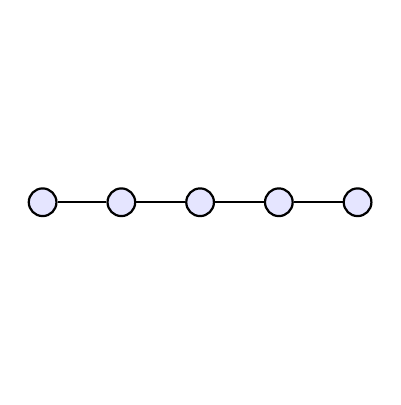
\begin{tikzpicture}[thick,main node/.style={circle,fill=blue!10,draw,minimum size=10pt}]
  	\node[main node] at (0,0) (1) {};
  	\node[main node] at (1,0) (2) {};
  	\node[main node] at (2,0) (3) {};
  	\node[main node] at (3,0) (4) {};
  	\node[main node] at (4,0) (5) {};
  	
  	\node[] at (0,-2.1) {};
  	\node[] at (0,2.1) {};
  	
  	
  	\path[-,every node/.style={font=\sffamily\Large}]
  	(1) edge node[left] {} (2)
  	(2) edge node[left] {} (3)
  	(3) edge node[left] {} (4)
  	(4) edge node[left] {} (5);
\end{tikzpicture}
}
\subfigure[Étoile]{
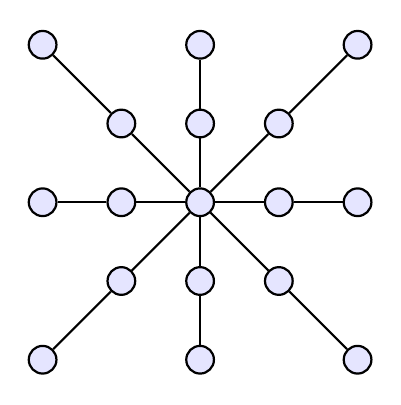
\begin{tikzpicture}[thick,main node/.style={circle,fill=blue!10,draw,minimum size=10pt}]
  	\node[main node] at (0,0) (1) {};
  	\node[main node] at (1,0) (2) {};
  	\node[main node] at (2,0) (3) {};
  	\node[main node] at (3,0) (4) {};
  	\node[main node] at (4,0) (5) {};
  	
  	\node[main node] at (2,1) (6) {};
  	\node[main node] at (2,2) (7) {};
  	
  	\node[main node] at (2,-1) (8) {};
  	\node[main node] at (2,-2) (9) {};
  	
  	\node[main node] at (1,1) (10) {};
  	\node[main node] at (0,2) (11) {};
  	
  	\node[main node] at (1,-1) (12) {};
  	\node[main node] at (0,-2) (13) {};  
  	
  	\node[main node] at (3,1) (14) {};
  	\node[main node] at (4,2) (15) {};
  	
  	\node[main node] at (3,-1) (16) {};
  	\node[main node] at (4,-2) (17) {};    		
  	
  	\node[] at (0,-2.1) {};
  	\node[] at (0,2.1) {};
  	
  	\path[-,every node/.style={font=\sffamily\Large}]
  	(1) edge node[left] {} (2)
  	(2) edge node[left] {} (3)
  	(3) edge node[left] {} (4)
  	(4) edge node[left] {} (5)
  	
  	(3) edge node[left] {} (6)
  	(6) edge node[left] {} (7)
  	
  	(3) edge node[left] {} (8)
  	(8) edge node[left] {} (9)
  	
  	(3) edge node[left] {} (10)
  	(10) edge node[left] {} (11)
  	
  	(3) edge node[left] {} (12)
  	(12) edge node[left] {} (13)  	
 
   	(3) edge node[left] {} (14)
  	(14) edge node[left] {} (15) 
  	
  	(3) edge node[left] {} (16)
  	(16) edge node[left] {} (17);
\end{tikzpicture}
}
\subfigure[Arbre]{
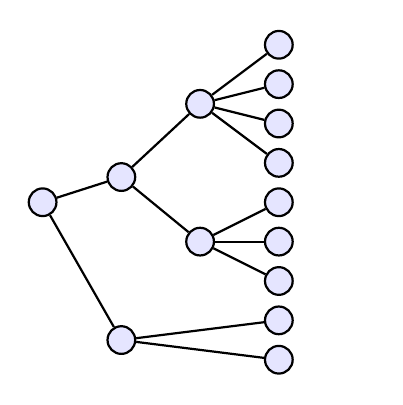
\begin{tikzpicture}[thick,main node/.style={circle,fill=blue!10,draw,minimum size=10pt}]
  	
  	\node[main node] at (0,0) (0) {};
  	\node[main node] at (1,0.32) (10) {};
  	\node[main node] at (1,-1.75) (11) {};
  	\node[main node] at (2,1.25) (20) {};
  	\node[main node] at (2,-0.5) (21) {};
  	\node[main node] at (3,2) (30) {};
  	\node[main node] at (3,1.5) (31) {};
  	\node[main node] at (3,1) (32) {};
  	\node[main node] at (3,0.5) (33) {};
  	\node[main node] at (3,0) (34) {};
  	\node[main node] at (3,-0.5) (35) {};
  	\node[main node] at (3,-1) (36) {};
  	\node[main node] at (3,-1.5) (37) {};
  	\node[main node] at (3,-2) (38) {};
  	
  	\node[] at (0,2.1) {};
  	\node[] at (4.1,-2.1) {};  	
  	
  	\path[-,every node/.style={font=\sffamily\Large}]
  	(0) edge node[left] {} (10)
  	(0) edge node[left] {} (11)
  	(10) edge node[left] {} (20)
  	(10) edge node[left] {} (21)
  	(11) edge node[left] {} (37)
  	(11) edge node[left] {} (38)
  	(20) edge node[left] {} (30)
  	(20) edge node[left] {} (31)
  	(20) edge node[left] {} (32)
  	(20) edge node[left] {} (33)
  	(21) edge node[left] {} (34)
  	(21) edge node[left] {} (35)
  	(21) edge node[left] {} (36);
\end{tikzpicture}
}
\subfigure[Boucle simple]{
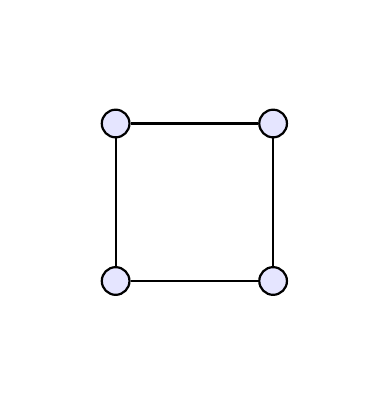
\begin{tikzpicture}[thick,main node/.style={circle,fill=blue!10,draw,minimum size=10pt}]
  	
  	\node[main node] at (1,1) (1) {};
  	\node[main node] at (1,-1) (2) {};
  	\node[main node] at (3,-1) (3) {};
  	\node[main node] at (3,1) (4) {};
  	
  	\node[] at (0,-2.1) {};
  	\node[] at (4,2.1) {};
  	
  	\path[-,every node/.style={font=\sffamily\Large}]
  	(1) edge node[left] {} (2)
  	(2) edge node[left] {} (3)
  	(3) edge node[left] {} (4)
  	(4) edge node[left] {} (1);
\end{tikzpicture}
}
\subfigure[Grille 2D]{
\begin{tikzpicture}[thick,main node/.style={circle,fill=blue!10,draw,minimum size=10pt}]
	\foreach \i in {0,...,4}{
		\pgfmathtruncatemacro{\x}{\i-2}
		\pgfmathtruncatemacro{\a}{\i-1}
		\foreach \j in {0,...,4}{
			\pgfmathtruncatemacro{\y}{\j-2}
			\pgfmathtruncatemacro{\b}{\j-1}
			
			\node[main node] at (\i,\j) (\i\j) {};
			
			\ifthenelse{\i>0}{
				\path[-] (\a\j) edge node[left] {} (\i\j);
			}
			
			\ifthenelse{\j>0}{
				\path[-] (\i\b) edge node[left] {} (\i\j);
			}			
		}
	}
\end{tikzpicture}
}
\subfigure[Connexité complète]{
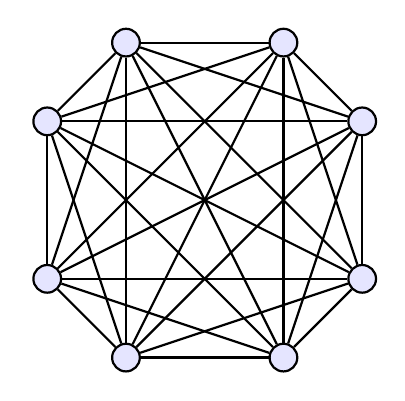
\begin{tikzpicture}[thick,main node/.style={circle,fill=blue!10,draw,minimum size=10pt}]
	\node[main node] at (0,1) (0) {};
	\node[main node] at (1,2) (1) {};
	\node[main node] at (3,2) (2) {};
	\node[main node] at (4,1) (3) {};
	\node[main node] at (4,-1) (4) {};
	\node[main node] at (3,-2) (5) {};
	\node[main node] at (1,-2) (6) {};
	\node[main node] at (0,-1) (7) {};
	
	
	\foreach \i in {0,...,6}{
		\foreach \j in {\i,...,7}{
			\path[-] (\i) edge node[left] {} (\j);
		}
	}
	
\end{tikzpicture}
}
